\documentclass[a4paper]{article}

%use the english line for english reports
%usepackage[english]{babel}
\usepackage[portuguese]{babel}
\usepackage[utf8]{inputenc}
\usepackage{indentfirst}
\usepackage{graphicx}
\usepackage{subfig}
\usepackage{verbatim}
\usepackage{listings} 
\usepackage{multicol}

\begin{document}

\setlength{\textwidth}{16cm}
\setlength{\textheight}{22cm}

\title{\Huge\textbf{MOD X}\linebreak\linebreak\linebreak
\Large\textbf{Relatório Final}\linebreak\linebreak
\linebreak\linebreak

\includegraphics[scale=0.1]{./images/feup-logo.png}\linebreak\linebreak
\linebreak\linebreak
\Large{Mestrado Integrado em Engenharia Informática e Computação} \linebreak\linebreak
\Large{Programação em Lógica}\linebreak
}

\author{\textbf{Grupo Mod X\_3:}\\
António Manuel Vieira Ramadas - 201303568 \\
Rui Miguel Teixeira Vilares - 201207046 \\
\linebreak\linebreak \\
 \\ Faculdade de Engenharia da Universidade do Porto \\ Rua Roberto Frias, s\/n, 4200-465 Porto, Portugal \linebreak\linebreak\linebreak
\linebreak\linebreak\vspace{1cm}}

\maketitle
\thispagestyle{empty}

%************************************************************************************************
%************************************************************************************************

\newpage

%Todas as figuras devem ser referidas no texto. %\ref{fig:codigoFigura}
%
%%Exemplo de código para inserção de figuras
%%\begin{figure}[h!]
%%\begin{center}
%%escolher entre uma das seguintes três linhas:
%%\includegraphics[height=20cm,width=15cm]{path relativo da imagem}
%%\includegraphics[scale=0.5]{path relativo da imagem}
%%\includegraphics{path relativo da imagem}
%%\caption{legenda da figura}
%%\label{fig:codigoFigura}
%%\end{center}
%%\end{figure}
%
%
%\textit{Para escrever em itálico}
%\textbf{Para escrever em negrito}
%Para escrever em letra normal
%``Para escrever texto entre aspas''
%
%Para fazer parágrafo, deixar uma linha em branco.
%
%Como fazer bullet points:
%\begin{itemize}
	%\item Item1
	%\item Item2
%\end{itemize}
%
%Como enumerar itens:
%\begin{enumerate}
	%\item Item 1
	%\item Item 2
%\end{enumerate}
%
%\begin{quote}``Isto é uma citação''\end{quote}

%%%%%%%%%%%%%%%%%%%%%%%%%%

\section*{Resumo\newline}

No âmbito da unidade curricular Programação em Lógica, foi-nos proposto desenvolver um jogo em linguagem PROLOG. Esse jogo, denomina-se MOD X e é bastante recente, tendo sido criado este ano.

O PROLOG é uma linguagem funcional e não uma linguagem procedimental. Assim, trabalhar nesta linguagem de programação foi um maiores desafios, tendo em conta a diferença que apresenta em relação com outras, tipicamente mais utilizadas.  

O esforço e o trabalho em equipa foram essenciais para resolver os problemas que foram surgindo. No entanto, reforçamos a importância das aulas teóricas, onde a matéria era exposta com clareza e permite uma mais fácil adaptação ao funcionamento e à essência dos objetivos propostos.

Através da cooperação e da forma objetiva que o trabalho foi elaborado, foi possível chegar a um resultado final simples, robusto, eficiente e apelativo. A execução em linha de comandos consegue ser clara e facilmente interpretada pelo utilizador comum. 

Em suma, considera-se o trabalho realizado de extrema importância para consolidar, mais facilmente, os conceitos abordados na aula. Os trabalhos práticos são sempre uma mais valia para adquirir conhecimento sólido, de uma forma direta e apelativa. 

\newpage
%%%%%%%%%%%%%%%%%%%%%%%%%%

%%\section*{Índice\newline}

\tableofcontents

\newpage

%%%%%%%%%%%%%%%%%%%%%%%%%%

\section{Introdução\newline}

Este trabalho foi realizado no âmbito da unidade curricular de Programação em Lógica, do curso Mestrado Integrado em Engenharia Informática e Computação. Inicialmente, foram disponibilizados vários jogos com o intuito de serem desenvolvidos em Prolog. 

A escolha recaiu no MOD X, essencialmente porque o seu mecanismo de jogo é compreendido com facilidade, utiliza um tabuleiro típico e apenas possui dois tipos de peças de jogo. Entenda-se por tabuleiro típico, um tabuleiro quadrado, semelhante ao utilizado nas damas.

Uma partida disputada entre dois jogadores, exige um bom conhecimentos sobre as regras de jogo e uma estratégia definida, adequada às próprias regras. Assim, este é um típico jogo de tabuleiro, onde a prática mental é exigida e testada em cada movimento.

O principal objetivo da realização deste trabalho prende-se na aplicação dos conceitos abordados nas aulas, tanto teóricas como práticas. A realização de um trabalho prático é sempre mais estimulante e adequada para aprender uma linguagem de programação.

Ao longo do relatório, procura-se contextualizar este jogo, abordado as suas regras, objetivos e componentes. É importante também descrever a implementação lógica do jogo em Prolog, seja ao nível de representação do estado do jogo, da visualização do tabuleiro, da lista de jogadas válidas, da execução de jogadas, da avaliação do tabuleiro, das condições finais de jogo e da forma de jogar do computador. A interface com o utilizador é descrita detalhadamente, facilitando a sua utilização e compreensão. A conclusão, a bibliografia e os anexos têm também uma presença chave neste relatório. 


\newpage

%%%%%%%%%%%%%%%%%%%%%%%%%%
\section{O Jogo MOD X\newline}

\subsection{Contextualização}
O MOD X é um jogo de tabuleiro, criado em 2015, recomendado para jogadores com mais de 15 anos de idade.
É um jogo de estratégia, divertido e fácil de aprender.
Cada partida reúne 2 a 4 jogadores e tem a duração prevista de 20 a 30 minutos. 

\subsection{Componentes do jogo}
\begin{itemize}
	\item 1 Tabuleiro 8x8;
	\item 56 peças de jogo em formato X (14 em cada cor);
	\item 72 marcadores de pontuação (18 em cada cor);
	\item 5 peças \textit{Joker} em formato X (brancas);
\end{itemize}

\begin{figure}[h!]
	\begin{center}
		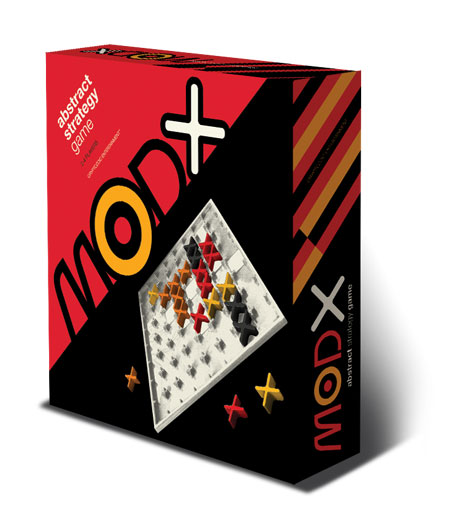
\includegraphics[scale=0.3]{./images/modx_box.jpg}
		\caption{Caixa do MOD X}
		\label{fig:1}
	\end{center}
\end{figure}

\subsection{Objetivo do jogo}

O objetivo deste jogo é criar padrões com peças coloridas (vermelho, preto, amarelo ou laranja).
Pretende-se assim, formar o maior número de padrões possível, de forma a conseguir a melhor pontuação.
O vencedor é o jogador com mais pontos.
Evidentemente, é também suposto bloquear os adversários de modo que não consigam construir esses padrões.  

\subsection{Regras}

\begin{itemize}
	\item Define-se a ordem dos jogadores, cada um escolhe a cor das suas peças e define-se o limite de pontos;
	\item Cada jogador inicia o jogo com 14 peças e 18 marcadores;
	\item Os \textit{Jokers} são dispostos inicialmente de forma aleatória no tabuleiro; 
	\item No seu turno, cada jogador coloca uma peça no tabuleiro, em qualquer posição livre;
	\item Os padrões utilizados para ganhar pontos são o ''X'', o ''+'' e o ''cinco em linha'';
	
	\begin{figure}[h!]
		\begin{center}
			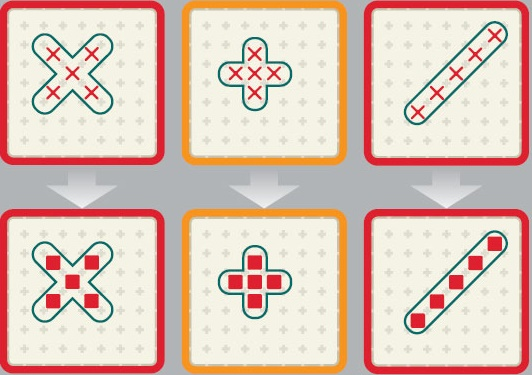
\includegraphics[scale=0.4]{./images/modx_score.jpg}
			\caption{Padrões usados}
			\label{fig:2}
		\end{center}
	\end{figure}
	
	\item O jogador pode usar os \textit{Jokers} para formar padrões, como se das suas próprias peças se tratassem;
	\item Quando um padrão é formado, retiram-se as peças de jogo e introduzem-se marcadores nessas posições. As peças de jogo podem agora voltar a ser utilizadas e as casas com marcadores também;
	\item Cada marcador colocado corresponde a um ponto;
	\item Caso tenha sido usado um \textit{Joker} para formar um padrão, nessa posição não é introduzido um marcador. O \textit{Joker} é agora colocado numa posição ao critério do jogador. Atenção, o \textit{Joker} não pode ser usado para formar um novo padrão de imediato; 
	
	\begin{figure}[!h]
		\centering
		\subfloat[Peças]{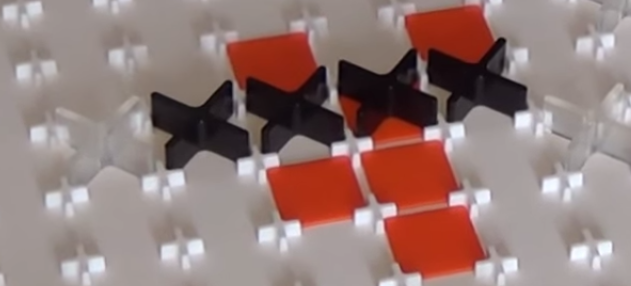
\includegraphics[width=0.3\textwidth]{./images/padroesPretos.png}\label{fig:3}}
		\hfill
		\subfloat[Marcadores]{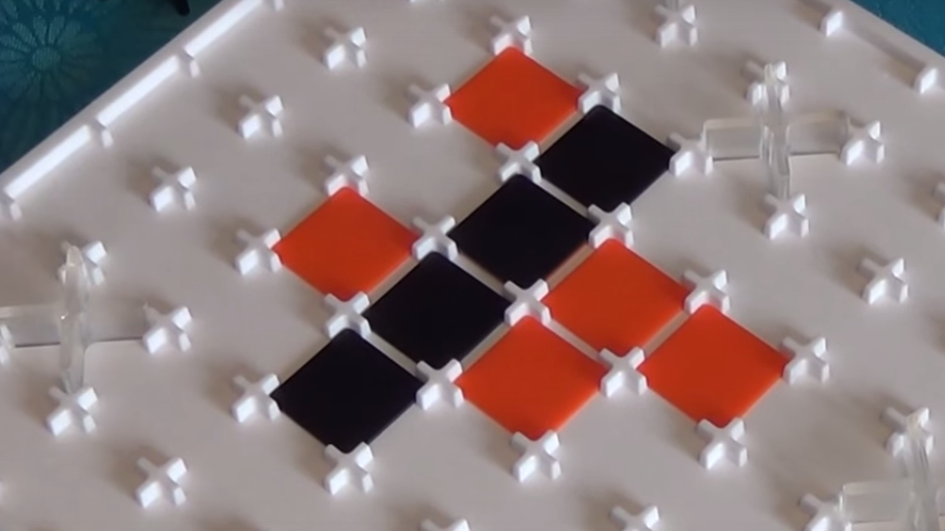
\includegraphics[width=0.3\textwidth]{./images/padroesPretosMarcadores.png}\label{fig:4}}
		\caption{Substituição das peças por marcadores}
	\end{figure}
	
	\item O primeiro jogador a atingir o número de pontos, determinado inicialmente, é o vencedor;
	\item O jogo pode também acabar quando um jogador já não dispõe de peças ou marcadores. Nesse caso, ganha o jogador com mais pontos até ao momento;
	

	
\end{itemize}

\newpage
%%Cada jogador inicia o jogo com 14 peças e 18 marcadores.
%%Inicialmente, define-se a ordem dos jogadores e escolha das peças por parte dos jogadores.  
%%No seu turno, um jogador coloca uma peça no tabuleiro, com o objetivo de criar padrões específicos, que se traduzem em pontos.
%%Os padrões utilizados para ganhar pontos são o ''X'', o ''+'' e o ''cinco em linha''.

%%Existem umas peças de cor branca, dispostas inicialmente de forma aleatória, chamadas Jokers. O jogador pode usar essas peças para formar padrões, como se tratassem das suas próprias peças.

%%É suposto bloquear os adversários de modo que não consigam construir esses padrões\footnote{https://www.cryptozoic.com/games/mod-x}.

%%No final, o primeiro jogador a atingir um certo número de pontos, determinado inicialmente pelo número de jogadores, é o vencedor.
%%O jogo pode também terminar quando um jogador terminar com as suas peças ou marcadores.
%%Nesse caso, o jogo termina imediatamente e ganha o jogador com mais pontos até ao momento.


%%%%%%%%%%%%%%%%%%%%%%%%%%
\section{Lógica do Jogo\newline}


\subsection{Representação do Estado do Jogo\newline}

O jogo é representado por uma lista de seis elementos. O objetivo desta estratégia é armazenar a informação do estado de jogo numa única lista. O primeiro elemento dessa lista corresponde ao estado atual do tabuleiro. O segundo elemento da lista corresponde a uma lista com a informação à cerca das peças disponíveis pelos jogadores. O terceiro elemento determina qual o jogador do turno atual. O quarto elemento da lista corresponde ao modo de jogo, do desafio em curso. O quinto elemento corresponde ao número de pontos com que o jogo deve terminar. Finalmente, o último elemento, corresponde ao nível de dificuldade do computador, quando é necessário. 

Na representação exterior, ou seja, quando o tabuleiro é visualizado pelo utilizador, usamos as seguintes propriedades:
\begin{multicols}{2}
	\begin{itemize}
		\item Peças de jogo:
		\begin{itemize}
			\item espaço em branco = livre (vazio)
			\item 0 = \textit{Joker} (transparente)
			\item 1 = jogador 1
			\item 2	= jogador 2
		\end{itemize}
		
		\columnbreak
		
		\item Marcadores:
		\begin{itemize}
			\item espaço em branco = vazio
			\item * = marcador do jogador 1
			\item : = marcador do jogador 2
		\end{itemize}
	\end{itemize}
\end{multicols}
	
Na representação interna, ou seja, nos dados armazenados pelo computador, usamos a seguinte sintaxe:
\begin{multicols}{2}
	\begin{itemize}
		\item Peças de jogo:
		\begin{itemize}
			\item -1 = livre (vazio)
			\item 0 = \textit{joker} (transparente)
			\item 1 = jogador 1
			\item 2 = jogador 2
		\end{itemize}
		\item Marcadores:
		\begin{itemize}
			\item -1 = vazio
			\item 11 = base do jogador 1
			\item 22 = base do jogador 2
		\end{itemize}
	\end{itemize}
\end{multicols}


\subsection{Visualização do Tabuleiro\newline}

A visualização do tabuleiro em modo de texto é feita através da composição de caracteres ASCII, como visto anteriormente. Para este efeito, foram desenvolvidos um conjunto de predicados. 

O predicado principal é:
\begin{itemize}
	\item \textbf{printBoard(Board)}: recebe uma lista descritiva das peças que constituem o tabuleiro e imprime-o;
\end{itemize}

Os predicados auxiliares são:
\begin{itemize}
	
	\item \textbf{printBoardAux(Board, CurrentNumberVertical)}: chamada auxiliar de \textit{printBoard} que desenha \textit{(Board.length mod 8)} vezes;	
	\item \textbf{printHorizontalLine(NumberOfDashes)}: imprime o número de travessões horizontais pretendido;
	\item \textbf{printBlock(Line)}: imprime todos os blocos de uma determinada linha (horizontal);
	\begin{itemize}
		\item \textbf{printLine1(' ', Tile)}: imprime a primeira linha do bloco;
		\item \textbf{print1(' ', Tile)}: predicado auxiliar de \textit{printLine1}, usada para a chamada recursiva;
		\item \textbf{printLine2(' ', Tile)}: imprime a segunda linha do bloco;
		\item \textbf{print2(' ', Tile)}: predicado auxiliar de \textit{printLine2}, usada para a chamada recursiva;
		\item \textbf{printLine3(' ', Tile)}: imprime a terceira linha do bloco;
		\item \textbf{print3(' ', Tile)}: predicado auxiliar de \textit{printLine3}, usada para a chamada recursiva;
		\item \textbf{toPrintMiddle(N)}: verifica se 
		\begin{math}
			N>0 \wedge N<8;
		\end{math}
		\item \textbf{printBeginning(\_)}: imprime o travessão vertical da primeira linha do bloco;
		\item \textbf{printMiddle(\_)}: imprime o travessão vertical da segunda linha do bloco;
		\item \textbf{printEnd(\_)}: imprime o travessão vertical da terceira linha do bloco;
	\end{itemize}
	\item \textbf{convertCode([Cross\textbar Tile], X, Y)}: traduz o átomo em peça de jogo;
	\begin{itemize}
		\item \textbf{convertCodeAux(Cross, [Tile\textbar \_], X, Y)}: predicado auxiliar de \textit{convertCode};
		\item \textbf{translateCodeToChar(X, Y)}: traduz o código X para o código Y;
	\end{itemize}
	\item \textbf{printInfo(\_)}: apresenta informação à cerca da representação do jogo;
	
	\begin{figure}[h!]
		\begin{center}
			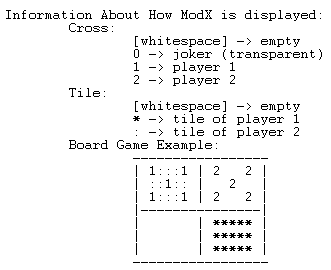
\includegraphics[scale=0.7]{./images/info.png}
			\caption{Informação geral apresentada}
			\label{fig:5}
		\end{center}
	\end{figure}
	
\end{itemize}

\subsection{Lista de Jogadas Válidas\newline}

No MOD X não faz sentido ser apresentada uma lista de jogadas válidas, porque uma jogada é sempre válida desde que a célula esteja vazia. Assim, caso esta funcionalidade fosse implementada, limitaria-se a apresentar uma lista com todas as células vazias. No entanto, essa condição é perfeitamente visível através da observação do tabuleiro e por isso é perfeitamente dispensável.

Apesar de existirem jogos de tabuleiro em que uma peça só pode ser movida mediante algumas restrições, isso não acontece no MOD X. Aqui, o jogador tem toda a liberdade de colocar uma nova peça numa posição vazia do tabuleiro.

O predicado que verifica se uma determinada célula está vazia é o \textbf{checkValidPosition(Board, Row, Col)}.    

\subsection{Execução de Jogadas\newline}

Em cada turno, o jogador introduz as coordenadas do tabuleiro onde pretende introduzir a peça através do predicado \textbf{putPlayerPiece(Board, Player, NewBoard)}. Esse predicado verifica se o estado da célula do tabuleiro, correspondente às coordenadas introduzidas, está vazia. Essa verificação é efetuada pelo predicado \textbf{checkValidPosition(Board, Row, Col)} e caso falhe, é pedido ao jogador para introduzir outras coordenadas. Assim que sejam introduzidas umas coordenadas que correspondam a uma célula vazia, a peça é colocada.

A peça \textit{Joker} merece especial enfoque, porque em caso de se formar um padrão com ela, têm que se recolocadas. No entanto, em caso de recolocação, as coordenadas de destino têm que corresponder a uma posição vazia e o \textbf{Joker} não pode ser utilizado para formar novamente um padrão. Assim, o predicado \textbf{putJoker(Board, NewBoard)} é responsável por colocar o \textit{Joker} numa nova posição e os predicados \textbf{checkValidPosition(Board, Row, Col)} e \textbf{checkPatern(Board, Row, Col)} responsáveis pelas respetivas verificações, mencionadas anteriormente. 

Finalmente, o predicado changePlayer(Game, NewGame) responsabiliza-se por alternar os turnos entre jogadores, depois de cada jogada estar completa.

\subsection{Avaliação do Tabuleiro\newline}

A avaliação do tabuleiro é efetuada no final de cada turno. Assim, depois de cada peça colocada no tabuleiro, ele é analisado completamente, verificando-se a existência de algum padrão. O predicado \textbf{checkAll(Board, Piece, NewBoard)} é responsável por essa verificação.

Caso algum padrão tenha sido formado, o devido ajuste ao tabuleiro é efetuado pelo predicado \textbf{fixBoard(Board, NewBoard, Game, NewGame)}. Atenção que o número de \textit{Jokers} é sempre analisado depois da formação de um padrão, para isso, recorremos ao predicado \textbf{assertNumJokers(Board, NewBoard)}.

\subsection{Final do Jogo\newline}

O predicado \textbf{playGame(Game)} é usado várias vezes para o normal funcionamento do programa. Associado à primeira declaração deste predicado, está o predicado \textbf{checkEndConditions(Game)}, que falha caso tenha sido encontrada uma condição de fim. 

O jogo termina quando o número final de pontos, estabelecido inicialmente, é atingido ou quando o número de peças ou marcadores chega a zero. Para verificar essas condições, são usados os predicados: \textbf{checkPointsEnd(Game)}, \textbf{checkPiecesEnd(Game)} e \textbf{checkMarkersEnd(Game)}.

O segundo predicado \textbf{playGame(Game)}, termina o jogo e declara que é o vencedor.

\subsection{Jogada do Computador\newline}

A forma mais adequada para proceder à implementação desta funcionalidade, seria através do algoritmo Minimax. No entanto, como isso ultrapassa os objetivos da unidade curricular, decidimos criar um algoritmo \textit{smart} que é responsável pelas jogadas do computador. 

O predicado \textbf{pcSmartMoveAlgorithm(Board, Player, NewBoard, Game)} cria 20 tabuleiros e avalia-os, escolhendo a melhor opção, ou seja, a que gera mais pontos. Cada um desses tabuleiros é avaliado individualmente, sendo calculada a pontuação resultante de cada um deles. A melhor opção é escolhida.

Além deste nível de jogo, está também disponível o modo \textit{Random}. Este nível de jogo, usado em turnos do computador, simplesmente coloca a peça numa posição aleatória.

Dependendo do nível de jogo definido pelo utilizador, o predicado \textbf{pcRandomMove(Game, NewGame)} ou \textbf{pcSmartMove(Game, NewGame)} são utilizados.

\newpage
%%%%%%%%%%%%%%%%%%%%%%%%%%

\section{Interface com o Utilizador\newline}

A interface de linha de comandos permite uma fácil utilização do programa. Os menus são simples e as opções são claras, permitindo ao utilizador selecionar a opção pretendida, tendo atenção a possíveis erros de \textit{input}.  

\begin{figure}[!h]
	\centering
	\subfloat[Main Menu]{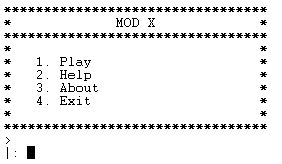
\includegraphics[width=0.3\textwidth]{./images/mainMenu.jpg}\label{fig:6}}
	\hfill
	\subfloat[Game Mode]{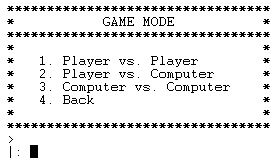
\includegraphics[width=0.3\textwidth]{./images/gameMode.jpg}\label{fig:7}}
	\caption{Escolha de modo de jogo}
\end{figure}

Ao longo da execução do programa, o ecrã vai sendo "limpo", através do predicado \textbf{cleanConsole}. Na prática o ecrã não é apagado, apenas são introduzidos espaços em branco para tornar a apresentação do jogo mais agradável.

\begin{figure}[!h]
	\centering
	\subfloat[Help Menu]{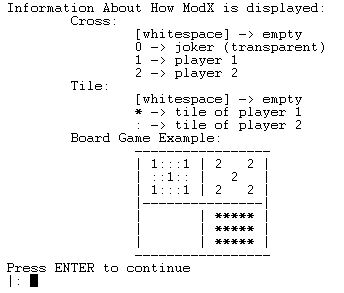
\includegraphics[width=0.3\textwidth]{./images/help.jpg}\label{fig:8}}
	\hfill
	\subfloat[About Menu]{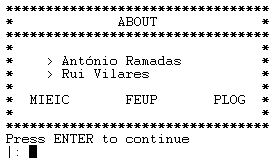
\includegraphics[width=0.3\textwidth]{./images/about.jpg}\label{fig:9}}
	\caption{Outras opções do menu principal}
\end{figure}



Em cada turno, é apresentado o tabuleiro e a informação associada ao jogador atual. Caso seja o turno do jogador, é pedido para serem introduzidas as coordenadas para inserir a peça. Caso seja o turno do computador, pede-se para pressionar ENTER e a peça é adicionada. 

\begin{figure}[h!]
	\begin{center}
		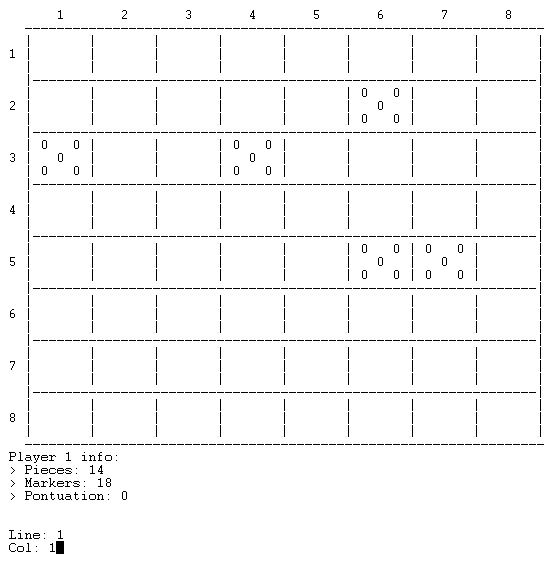
\includegraphics[scale=0.7]{./images/game.jpg}
		\caption{Exemplo de jogo}
		\label{fig:10}
	\end{center}
\end{figure}

\clearpage

%%%%%%%%%%%%%%%%%%%%%%%%%%

\section{Conclusões\newline}

Apesar do exaustivo trabalho que a implementação do jogo MOD X exigiu, o resultado final e os conhecimentos adquiridos ao longo da sua implementação são considerados bastante positivos. Considera-se que todos os objetivos propostos inicialmente foram cumpridos, bem como os critérios estabelecidos inicialmente pelos docentes.

A implementação do MOD X foi um desafio encarado com frontalidade. Importa referir que algumas partes do processo de desenvolvimento mostraram-se complicadas de realizar. Nem sempre a linguagem foi um problema, como seria de esperar. Em alguns casos, as regras próprias do jogo foram a verdadeira entrave. 

Como dito anteriormente, todos os objetivos e requisitos propostos foram cumpridos. No entanto, há sempre espaço para melhorias, nomeadamente na implementação do algoritmo \textit{smart}. Poderia ser implementado uma forma anti-jogo, impossibilitando o adversário de formar padrão.  

Concluindo, o Prolog é uma linguagem que requer um pensamento lógico. A utilização desta linguagem acabou por ser uma agradável surpresa e por isso, consideramos que os conceitos adquiridos serão benéficos no futuro.

\newpage

%%%%%%%%%%%%%%%%%%%%%%%%%%

\section*{Bibliografia\newline}

\begin{itemize}
	\item https://boardgamegeek.com/boardgame/131387/mod-x
	\item https://www.cryptozoic.com/games/mod-x
	\item https://youtu.be/pto-7O618rI
	\item Apresentações utilizadas nas aulas teóricas
	\item Livro: Sterling, Leon; The Art of Prolog
\end{itemize}

\newpage

%%%%%%%%%%%%%%%%%%%%%%%%%%

\section*{Anexos\newline}

Código fonte do projeto encontra-se na pasta MODX anexado junto deste relatório.

%%%%%%%%%%%%%%%%%%%%%%%%%%

\end{document}
